\documentclass[a4paper,11pt,openany,extrafontsizes,oneside,article]{memoir}

\usepackage{fontspec}

\setmainfont[Numbers=OldStyle]{Linux Libertine O}
\setsansfont[Numbers=OldStyle]{Linux Biolinum O}
%\setmonofont{Inconsolata}
\setmonofont[Scale=0.83]{Bitstream Vera Sans Mono}

\usepackage{polyglossia}
\setdefaultlanguage{english}

%\usepackage{graphicx}
\usepackage{xcolor}
%\usepackage{wrapfig}
%\usepackage{subfig}
%\usepackage{lettrine}
%\usepackage{tikz}
%\usepackage{amsmath,amssymb}

%\usepackage{pdfpages}

\usepackage{microtype}

%% Propriétés du document PDF
\usepackage[hidelinks]{hyperref}

\hypersetup{
  pdfauthor={Joseph Budin, Dimitri Lozeve},
  pdftitle={TDA TD5: Topological Persistence},
  pdfsubject={Report},
  pdfkeywords={report,tda,td5,topological,persistence},
  pdfpagemode=UseOutlines,
  pdfpagelayout=TwoColumnRight
}

\usepackage{minted}
\setminted[java]{linenos,stepnumber=5,autogobble,fontsize=\small}
\setminted[python]{linenos,stepnumber=5,autogobble,fontsize=\small}

%% Pour la classe memoir /!\

%% Marges
\setulmarginsandblock{3cm}{3cm}{*}
\setlrmarginsandblock{3cm}{3cm}{*}
\checkandfixthelayout

%% Numérotation des divisions logiques
\setsecnumdepth{subsection}
\maxsecnumdepth{subsection}

%% Profondeur de la ToC
\settocdepth{subsection}
\maxtocdepth{subsection}

%% Style des titres des divisions logiques
\setsecheadstyle{\Large\scshape}
\setsubsecheadstyle{\large\scshape}

%% style des environnements description
%\renewcommand*{\descriptionlabel}[1]{\hspace\labelsep
%  \normalfont\itshape #1}

%% épigraphes
%\setlength{\epigraphwidth}{0.5\textwidth}
%\epigraphtextposition{flushleftright}


\author{Joseph Budin \and Dimitri Lozeve}
\date{\today}
\title{\Huge TD5: Topological Persistence\\ \LARGE Report}



%%% Local Variables:
%%% mode: latex
%%% TeX-master: "report"
%%% End:


\begin{document}

%\pagestyle{Ruled}
\tightlists{}

\maketitle

%% Style de chapitre
% \chapterstyle{hangnum}

% \tableofcontents*

\chapter{Question 3: Complexity of the Reduction Algorithm}
\label{chap:q3}

\begin{minted}{java}
    void reduction() {
        // Reminder:
        // lowIndices stores the row index of the lowest non-zero entry for each column.
        // lowColumn[k] stores the index of the column which has its lowest entry at row k.

        // We loop through all columns
        for (int j = 0; j < this.n; j++) {
            int low = getLow(j);
            // While the column is not empty and there exists a previous column with the same pivot:
            while (low != -1 && lowColumn[low] != -1) {
                // We update the j-th column
                int i = lowColumn[low];
                reductColumns(i, j);
                // We compute the new pivot
                low = getLow(j);
            }
            // Final pivot
            lowIndices[j] = low;
            // If the column is non-empty, we complet lowColumn
            if (low != -1) {
                lowColumn[low] = j;
            }
        }
    }
\end{minted}

We have 3 loops. The \mintinline{java}|for| loop runs through all the
columns, so $m$ times, where $m$ is the number of simplices. The
\mintinline{java}|while| loop cycles through all previous columns, so
$\mathcal{O}(m)$ iterations. Finally, the method
\mintinline{java}|reductColumns| does a symmetric difference on the
$i$-th and $j$-th columns, and thus requires at most $m$
operations. Therefore, the total complexity of the reduction algorithm
is $\mathcal{O}(m^3)$.


\chapter{Questions 5-6: Classical Spaces}
\label{chap:q5}

The filtrations for the spheres in dimension $d$ are generated by the
following Python script:

\begin{minted}{python}
from itertools import combinations

if __name__ == "__main__":
    for d in range(11):
        f = open("sphere_"+str(d)+".txt", 'w')
        n = d + 2
        for i in range(1, n):
            simplices = set(combinations(range(n), i))
            for x in simplices:
                f.write(str(i-1) + " " + str(i-1) + " ")
                for j in range(len(x)):
                    f.write(str(x[j]) + " ")
                f.write("\n")
\end{minted}

The results corresponds to the ones obtained by hand in the exercise
session.


\chapter{Question 7: Timings}
\label{chap:q7}

\begin{tabular}{lrrrrr}
  filtration & number of simplices & creation time (s) & reduction time (s)
  & time / $m^3$ & time / $m\sqrt{m}$\\
  \hline
  A & 428,643 & 2.365 & 24.654 & 3.13E-13 & 8.78E-05 \\
  B & 108,161 & 6.93 & 1.319 & 1.04E-12 & 3.71E-05 \\
  C & 180,347 & 2.797 & 2.821 & 4.80E-13 & 3.68E-05 \\
  D & 2,716,431 & 162.546 & 263.103 & 1.31E-14 & 5.87E-05 \\
\end{tabular}

\begin{figure}[ht]
  \centering
  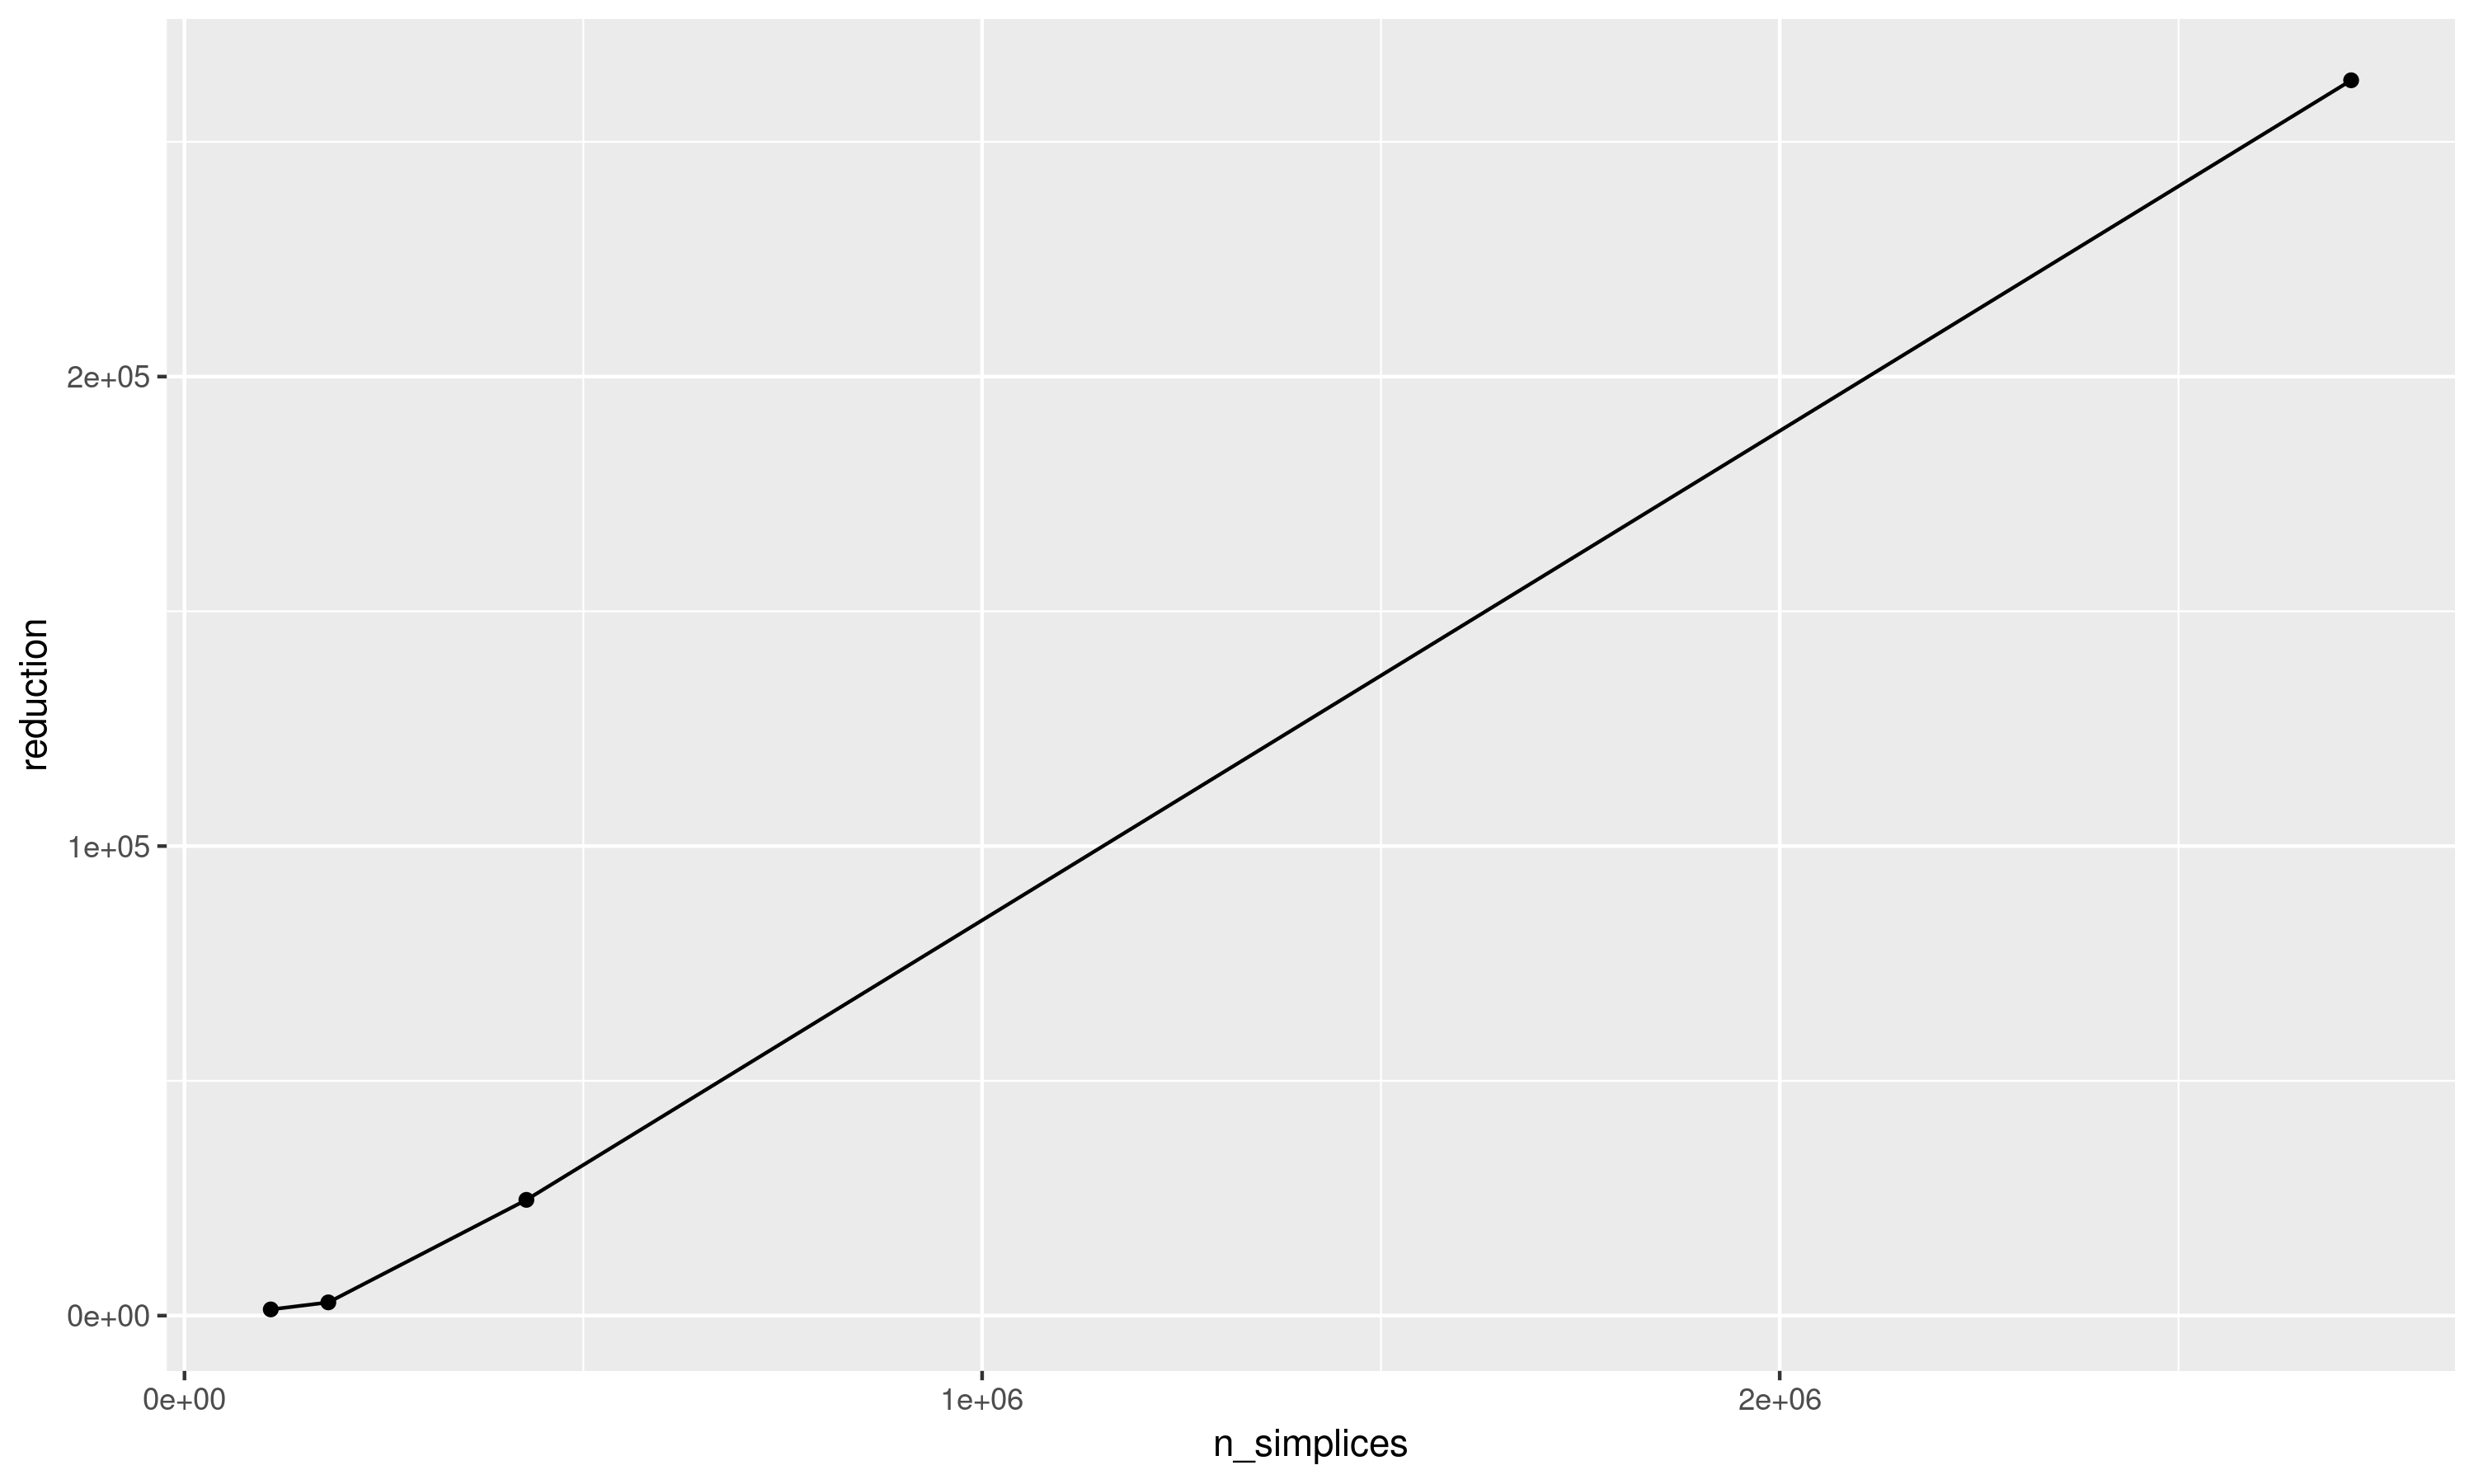
\includegraphics[width=\linewidth]{timings.png}
  \caption{Reduction time vs. number of simplices in the filtration}
  \label{fig:timings}
\end{figure}

In the table, we show the time that the program uses to create the
(sparse) matrix and to reduce it. We then try to test if it is indeed
cubic in the number of simplices. Experimentally, we have a slightly
better complexity (around $\mathcal{O}(m^{1.5})$), probably due to the
fact that most columns are empty or that there are very few columns
with the same pivot.

\chapter{Question 8: Topological Structure}
\label{chap:q8}

\section{Filtration A}

This barcode corresponds to a sphere. If we visualize points on the
surface of a sphere, and balls slowly growing around them, we can
infer the good number of holes and voids to match the barcode.

First, there are many connected components, so in $H_0$ many
segments. After a while, all these components merge together, thus
reducing gradually the number of holes (i.e. the number of segments in
$H_1$).

When the last hole has disappeared, a single void appears (in
$H_2$). After some times, all the little ball have grown and this void
disappears, leaving no hole or void, and only one connectefd
component.

\section{Filtration B}

We apply the same reasoning. This time, the underlying topological
space is a set of 8 spheres, position at the vertices of a cube, and
tangent to each other. There is only one connected component, and
initially 5 holes (because there are 6 openings on the sides of the
cube formed by the sphere, but only 5 independant cycles). There are
also 8 voids (the interiors of the spheres).

When every hole has disappeared, a void appears in the inside of the
cube.

\section{Filtrations C and D}

These filtrations corresponds to a torus. Once the many connected
components have merged together, there are many holes on the
surface. The disappear progressively, leaving only the two independant
cycles on the surface of the torus.

Afterwards, the torus fills itself, making one of the cycles to
disappear, and simultaneously, the void inside disappears. (We have a
little bit of noise because the void does not fill itself immediately;
a lot of smaller voids appear and disappear very quickly.) Then the
central hole in the torus disappears also, and the torus has become a
single ball.


\end{document}



%%% Local Variables:
%%% mode: latex
%%% TeX-master: t
%%% End:
